\documentclass[../thesis/thesis.tex]{subfiles}
\begin{document}
 \chapter{Methods}
With a minimum viable prototype established, it now becomes possible to devise experimental scenarios to test against the project's goals. The project's adherence to the goals of Low-Cost and Non-Invasiveness have been evaluated previously, so in this section we will focus on the project's adherence to Reliability and Energy Efficiency goals.

\section{Reliability Testing}

With the prototype, it is now possible to utilize the prototype to gather both thermal and visual data in a synchronized format. This data can be collected and used to determine the effectiveness of the human counting algorithms used. Due to the prototype's technical similarly to Thermosense \cite{beltran2013thermosense}, a similar set of experimental conditions will be used, with a comparison against Thermosense being used as a benchmark. To this end, several experiments were devised, each of which had its data gathered and processed in accordance with the same general process, outlined in \Fref{fig:methods:flowchart}.

\begin{figure}
\centering
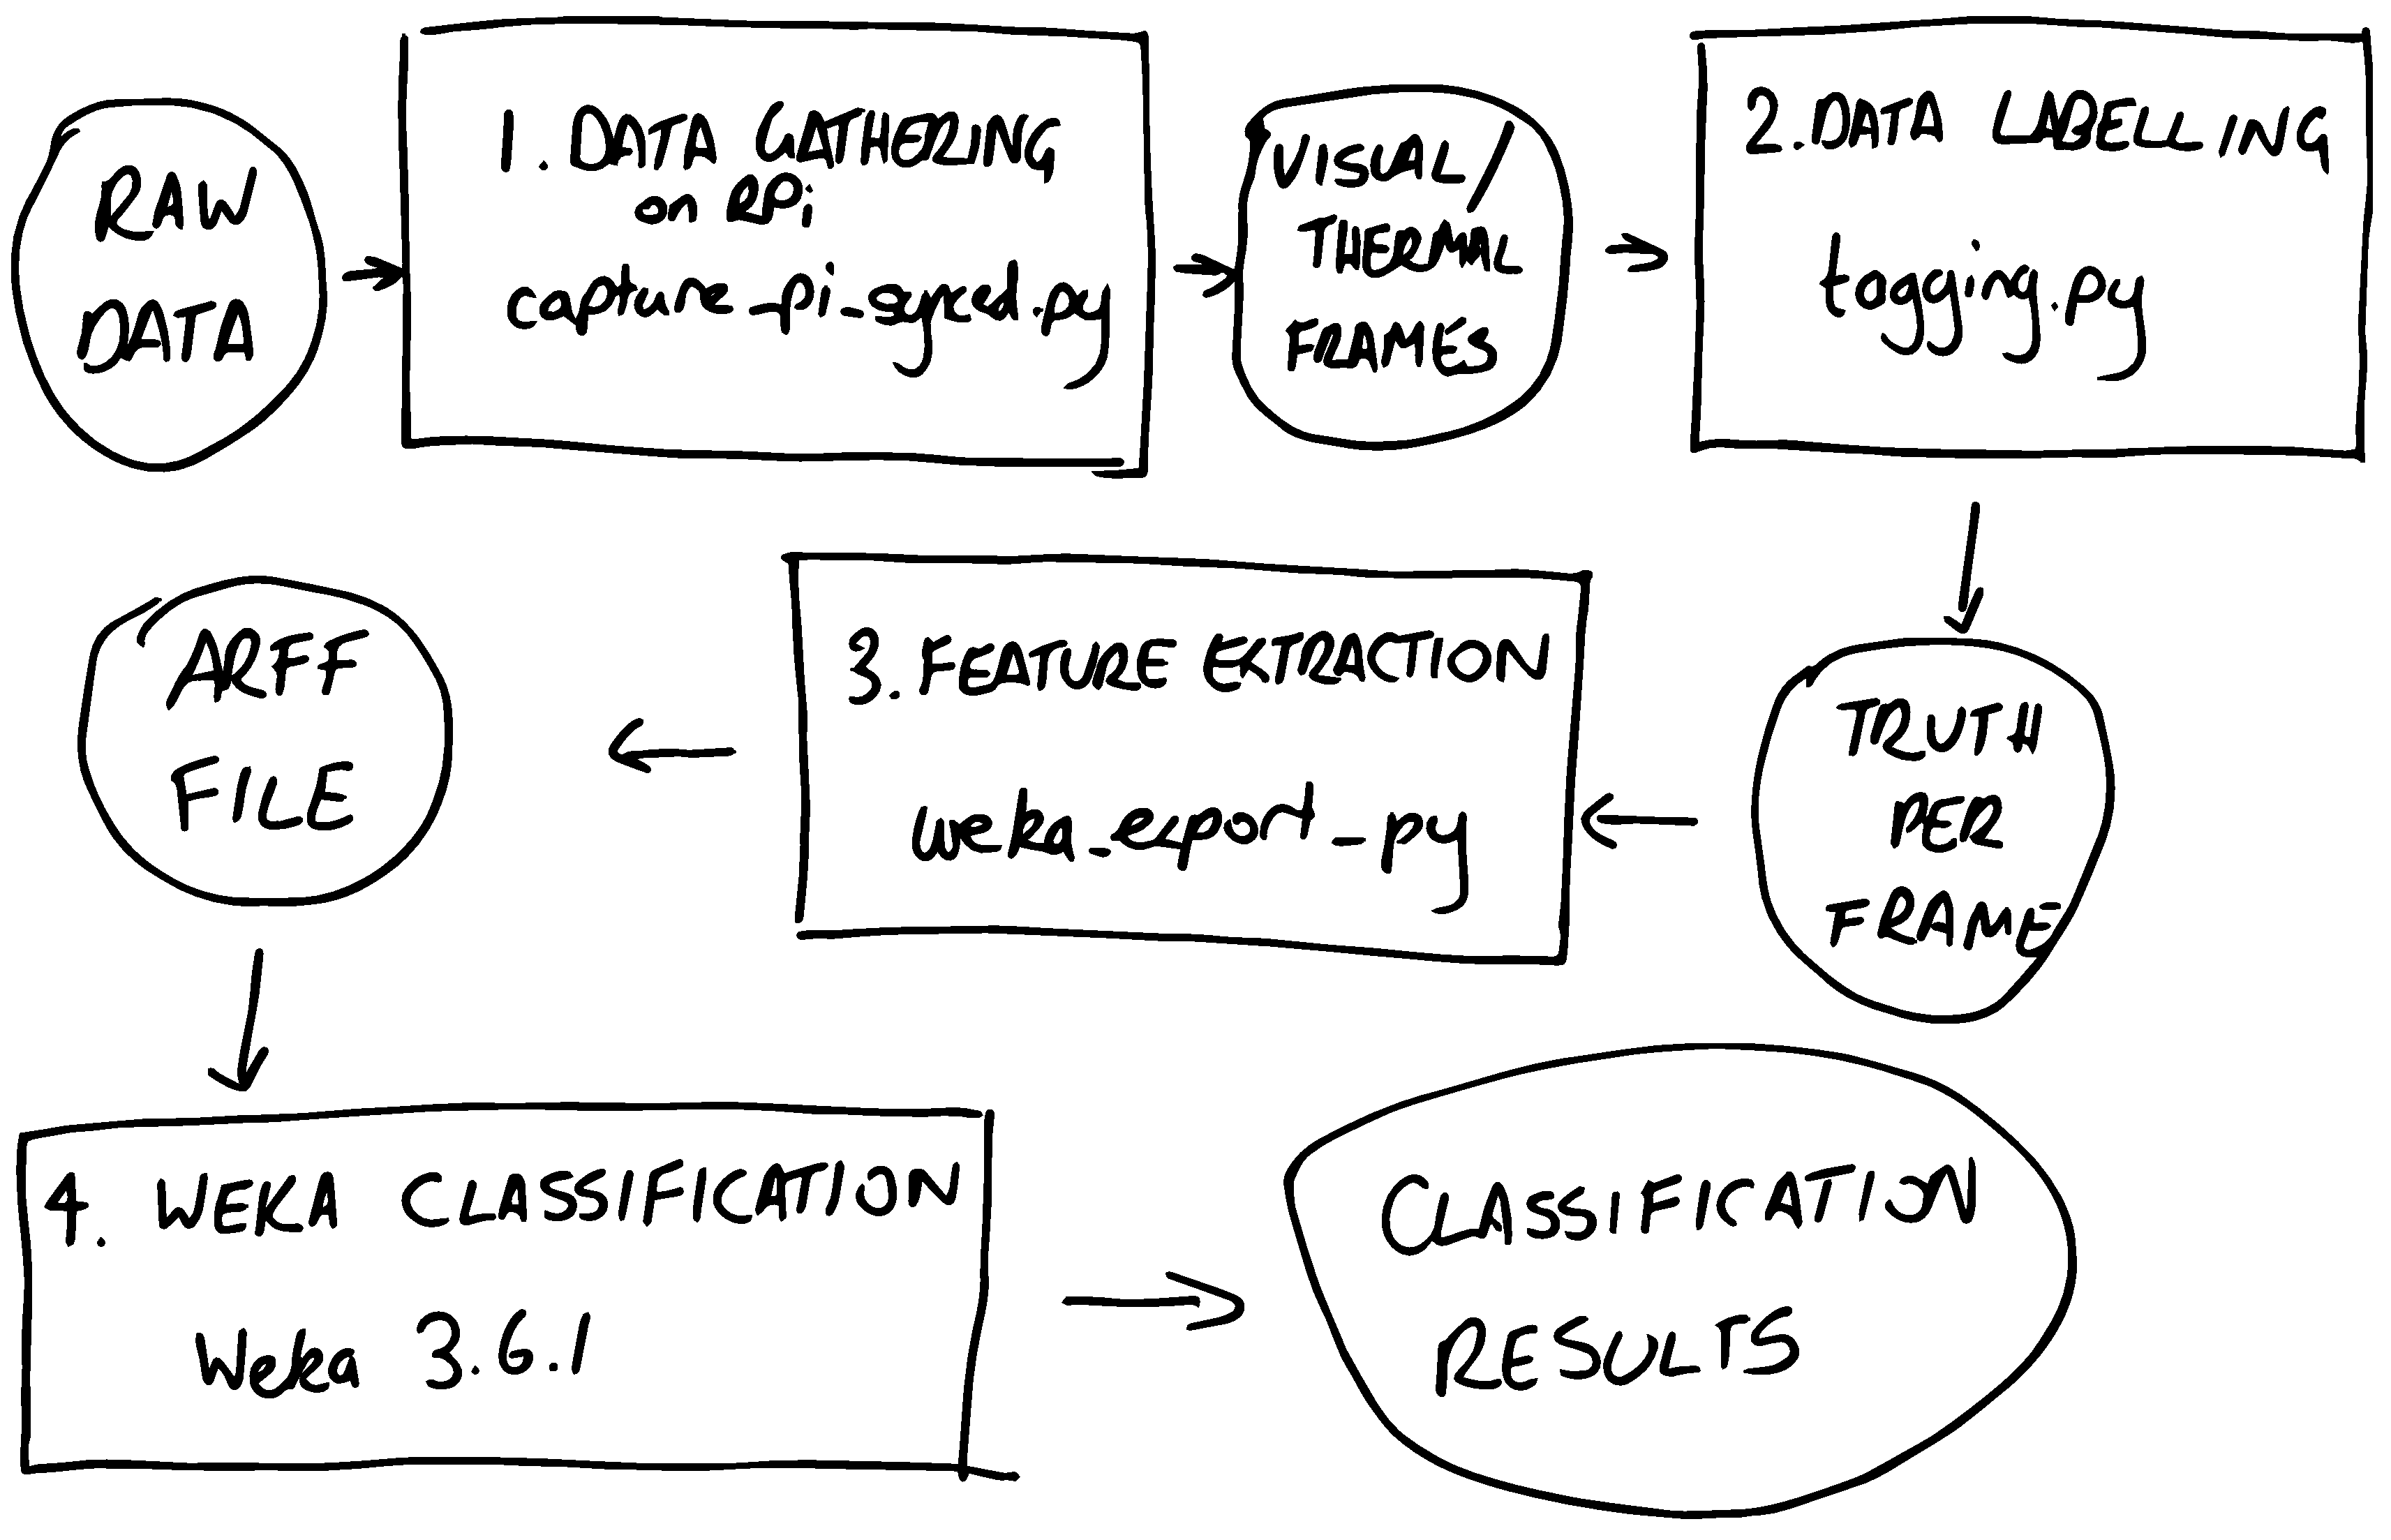
\includegraphics[width=0.95\textwidth]{../diagrams/temp/method-flowchart.pdf}
\caption{Flowchart of processing}
\label{fig:methods:flowchart}
\end{figure}

\subsection{Data gathering}
As the camera and the Arduino are directly plugged into the Raspberry Pi, all data capture is performed on-board through SSH, with the data being then copied of the Pi for later processing. To perform this capture, the main script used is \texttt{capture\_pi\_synced.py}.

\texttt{capture\_pi\_synced.py} takes two parameters on the command line; the name of the capture output, and the number of seconds to capture. By default, it always captures at 2Hz. The script initializes the \texttt{picamera} library, then passes a reference to it to the \texttt{capture\_synced} function within the \texttt{Visualizer} class. The class will then handle the sending of commands to the Arduino to capture data in concert with taking still frames with the Raspberry Pi's camera.

When the script runs, it creates a folder with the name specified, storing inside a file named \texttt{output\_thermal.hcap} containing the thermal capture, and a sequence of files with the format \texttt{video-\%09d.jpg}, corresponding to each visual capture frame.

\subsection{Data labeling}
Once this data capture is complete, the data is copied to a more powerful computer for labeling. The utility \texttt{tagging.py} is used for this stage. This script is passed the path to the capture directory, and the number of frames at the beginning of the capture that are guaranteed to contain no motion. This utility will display frame by frame each visual and thermal capture together, as well as the computed feature vectors (based on a background map created from the first $n$ frames without motion).

The user is then required to press one of the number keys on their keyboard to indicate the number of people present in this frame. This number will be recorded in a file called \texttt{truth} in the capture directory. The next frame will then be displayed, and the process continues. This utility enables the quick input of the ground truth of each capture, making the process more efficient.

\subsection{Feature extraction and data conversion}
% TODO: Explain classification

Once the ground truth data is available, it is now possible to utilize the data to perform various classification tests. For this, we use version 3.7.12 of the open-source Weka toolkit \cite{Weka}, which provides easy access to a variety of machine learning algorithms and the tools necessary to analyze their effectiveness.

To enable the use of Weka, we export the ground truth and extracted features to a Comma Seperated Value (CSV) file for processing. \texttt{weka\_export.py} takes two parameters, a comma-separated list of different experiment directories to pull ground truth and feature data from, and the number of frames at the beginning of each capture that can be considered as ``motionless.'' With this information, a CSV-file file is generated on which the heading indicating the attribute names is added for Weka to recognize.

\subsection{Running Weka Tests}
Once the CSV file is generated, it is then possible to open the file in Weka for processing. Weka provides a variety of algorithms, but we choose a specific subset of algorithms based on those present in the Thermosense paper \cite{beltran2013thermosense}, as well others that we believe adequately represent the different approaches to classification.

% TODO: Do I need equations for these explanations?
\subsubsection{Neural Networks}
An artificial neural network (ANN) uses neurons as a model for machine learning. A number of input neurons, in this case connected to the feature vectors, is fed into a network of neurons (the ``hidden layer''), each of which has an activation function which determines what set of inputs will make it fire. This network then connects to a number of output neurons which can be queried to determine the network's predicted result. In the nominal result case, there one neuron for each possible class, and in the numeric result case, there is one neuron without an activation function that outputs the raw numerical estimate. Neural networks can approximate functions of nearly any complexity with sufficient neurons in the correct topology, and are a quite common classification technique.

Thermosense uses a neural network with a hidden layer of five neurons, with a sigmoid activation function for the hidden layer and a linear activation function for the output layer. They test only the one, two and three person cases, relying on their \pir to detect the zero person case. They use 70\% of their data for training the neural net, 15\% for testing the net and the final 15\% for validating their results. Thermosense conducts tests interpreting the number of people as a numeric attribute.

We use Weka's ``MultilayerPerceptron'' neural network, which creates a hidden layer of $(\mathit{attributes} + \mathit{classes}) / 2$ (three) by default, however we manually reconfigure this to be one hidden layer of five neurons, like Thermosense. It uses a sigmoid activation function for all neurons, except in the case that a numerical answer is to be predicted, in which case like Thermosense, it uses a linear activation function for the output layer. As is standard, for validation we use a 10-fold cross-validation for our nominal approach, and attempt to replicate Thermosense's configuration as closely as possible for the numeric result. % TODO: Actually do this

\subsubsection{$k$-nearest Neighbors}
A $k$-nearest Neighbors (KNN) approach uses the topology of the training data as a means to classify future data. For each data point that requires classification, a majority vote of its $k$ nearest neighbors in the training data determines which class it belongs to. KNN is one of the simplest machine learning algorithms, and due to its classification method, is highly sensitive to classes that overlap. 

Thermosense uses 5-nearest Neighbors with the Euclidean distance between points. For determining the class label, higher weightings are given to training points inversely to their distance from the point being classified. Thermosense appears to use a nominal classification for their KNN.

We use Weka's ``iBk'' function to perform a KNN calculation, configuring \texttt{distanceWeighting} to be ``Weight by 1-distance'' and \texttt{KNN} to be 5, to make the classification as similar in function to the Thermosense approach as is possible. Thermosense does not specify what validation technique they used, so we elected to use a standard 10-fold cross-validation.

\subsubsection{Linear Regression}
A Linear Regression approach attempts to construct a linear equation to describe the relationship between a dependent variable (in this case, the number of people in the space), and a number of other indicator variables (in this case, the three feature vectors). Generally, the equation takes the form $y = m_1x_1 + ... + m_nx_n + c$, where each of the feature vectors is multiplied by a weight, and then a final number is added to provide the final prediction.

Thermosense uses a Linear Regression model of $y = \beta_A A + \beta_S S + \beta $, whereby $A$ is the number of active pixels, $S$ is the size of the largest connected component, and the $\beta$ values represent the corresponding coefficients. They opt to exclude the third feature, the number of connected components, as their testing indicates that excluding it minimizes the Root Mean Squared Error (RMSE) further. 

We use Weka's ``LinearRegression'' function, exclude the \texttt{numconnected} attribute from the feature vector list, to attempt to match this approach.


\subsubsection{Naive Bayes}
A Naive Bayes approaches uses a simple application of Bayes' probability theorem to construct a probability of a given value belonging to a given class taking into account what is already known about the distribution of each of the classes in the data set, and the classification of those points that surround the point needing classification. One of the disadvantages of the Naive Bayes approach (the source of its naivety) is that it assumes independence between each of the variables used for classification.

In our data, the assumption of independence of variables is not correct, as each of the features are slightly different representations of the same data. However, due to Naive Bayes' ubiquity and simplicity, it can be illuminating to see how well a very common but poorly suited classifier fares with our data set. Within Weka, we use the ``NaiveBayes'' function, which has little by way of configuration, thus is left in its default state.

\subsubsection{Support Vector Machines}
Support Vector Machines (SVM) attempt to classify data by trying to find a plane that best separates two classes in a higher dimensional space. They do this by determining ``support vectors,'' which are those data points that lie on the ``edge'' of the separation between classes, and then finding the plane that maximizes the margin between the two classes. We elected to test an SVM-based approach to determine if our data set is particularly suited to classification by SVMs.

For our purposes, we use Weka's ``SMO'' function, which implements the Sequential Minimal Optimization algorithm, an efficient and recent method of training SVMs. For datasets with more than two classes (such as ours), the ``one vs. one'' method is used, whereby an SVM is created for each pair of classes, and then a method of majority voting is used to determine which class is the ultimately correct one. % TODO: Need to cite SMO?

\subsubsection{Decision Trees}
A Decision Tree based approach uses the concept of a decision tree to create effectively a list of logical conditions which when met cause a data point to be classified as a specific class. Decision Tree classifiers generally use a partitioning approach whereby they split the data using a specific metric to maximize the tree's effectiveness. The advantages of Decision Trees are that they are considered to be ``white boxes,'' specifically meaning that the result that they generate is human readable. This is useful, as in addition to the classifier providing its prediction of which class suits the data best, the tree can also be inspected to determine if the decisions it has extrapolated appear to be sensible, and even tweaked by humans if necessary.

One quite common algorithm for generating decision trees is C4.5, which is implemented by the ``J48'' function in Weka. C4.5 uses a measure of information gain, a concept rooted in information theory and entropy, to determine when to create splits in the tree. There are few configurable parameters for this approach, and for those we use the Weka defaults.

\subsubsection{KStar}
The KStar (K*) algorithm presents a change to the normal $k$-nearest Neighbors algorithm, in which the distance used to compare similar points is not the Euclidean distance, but rather an entropic distance. This has several positive effects; it makes the algorithm more robust to missing values, and also it makes the classifier able to output a numeric result in addition to or instead of a classification into a nominal class.

We have decided to use K* as one of our classification algorithms as it presents an interesting and different approach, and also allows the investigation of KNN-like techniques in the numeric area. K* is present in Weka as ``KStar,'' and we will opt to use it in its default state.

\subsubsection{0-R}
0-R is our final classification algorithm. 0-R is a simple classifier that on nominal prediction will classify all new data as belonging to the category that was most common in the training data, and on numeric prediction will classify all new data as being the mean of all test data. A 0-R classifier, clearly, is not a serious classification technique, however it is useful in establishing a baseline from which to compare all other classification results.

In Weka, the 0-R classifier is known as ``ZeroR'' and accepts no parameters.

\subsubsection{Excluding Zero}
TODO: Talking about how there are two sets of data, that which includes the zero data, and that which excludes it and relies on the PIR to confirm zero. Pros and cons of these approaches.


\begin{landscape}
\begin{table}
\centering
\begin{tabular}{|p{50mm}|p{20mm}|p{125mm}|}
\hline
\textbf{Type} & \textbf{Attribute} & \textbf{Weka Class} \& \textbf{Parameters} \\ \hline

Neural Network (ANN) & {Nominal, \newline Numeric} & \texttt{weka.classifiers.functions.MultilayerPerceptron \newline -L 0.3 -M 0.2 -N 500 -V 15 -S 0 -E 20 -H 5} \\ \hline

$k$-nearest Neighbors (KNN) & Nominal, \newline Numeric & \texttt{weka.classifiers.lazy.IBk \newline -K 5 -W 0 -F \newline -A "weka.core.neighboursearch.LinearNNSearch -A \textbackslash"weka.core.EuclideanDistance -R first-last\textbackslash""} \\ \hline

Naive Bayes & Nominal & \texttt{weka.classifiers.bayes.NaiveBayes} \\ \hline

Support Vector Machine (SVM) & Nominal & \texttt{weka.classifiers.functions.SMO \newline -C 1.0 -L 0.001 -P 1.0E-12 -N 0 -V -1 -W 1 \newline -K "weka.classifiers.functions.supportVector.PolyKernel -C 250007 -E 1.0"} \\ \hline

Decision Tree & Nominal & \texttt{weka.classifiers.trees.J48 \newline -C 0.25 -M 2} \\ \hline

Entropy Distance & Nominal, \newline Numeric & \texttt{weka.classifiers.lazy.KStar \newline -B 20 -M a} \\ \hline % TODO: Check that entropy distance

Linear Regression & Numeric & \texttt{weka.classifiers.functions.LinearRegression \newline -S 0 -R 1.0E-8} \\ \hline

0-R & Nominal, \newline Numeric & \texttt{weka.classifiers.rules.ZeroR} \\ \hline
\end{tabular}
\caption{Weka parameters used for classifications}
\label{tab:methods:params}
\end{table}
\end{landscape}

For those tests that are ``nominal,'' the \texttt{npeople} attribute was interpreted as nominal using the ``NumericToNominal'' filter, which creates a class for each value deleted in \texttt{npeople}'s columns. For those tests that are ``numeric,'' \texttt{npeople} is left unchanged, as by default all CSV import attributes are interpreted as such. For all tests where not specifically instructed, we use 10-fold cross-validation to validate our results.

As the data we are using is based on real experiments, the number of frames which are classified as each class may be unbalanced, which could cause the classification results to be affected. To that end, for each classification technique, we both classify the data in its raw, unbalanced form, and we also uniformly re-sample the \texttt{npeople} parameter using \texttt{weka.filters.supervised.instance.Resample -B 1.0 -S 1 -Z 100.0} in the pre-processing stage.

To help maximize the efficiency of the classification task, we use the Weka Knowledge Flow constructor to generate an encompassing flow that accepts an input CSV file of the raw data, and performs all resampling, numeric and nominal classification, returning a text file with the results of each of the different classification techniques run. The knowledge flow's struture can be seen in \label{fig:methods:unifiedflow}. To enable maximum efficiency, the input and output elements of this flow are set to the environmental variables \texttt{UnifiedFlow.InputCSV} and \texttt{UnifiedFlow.OutputCSV}, a Jython script, \texttt{run\_flow.py}, then sets those environmental variables to input and output file names, then calls the flow using Weka's Java API. After this is complete, the script then runs a series of regexes on the output text data to generate summary spreadsheets with the relevant values.

\begin{landscape}
\begin{figure}
\centering
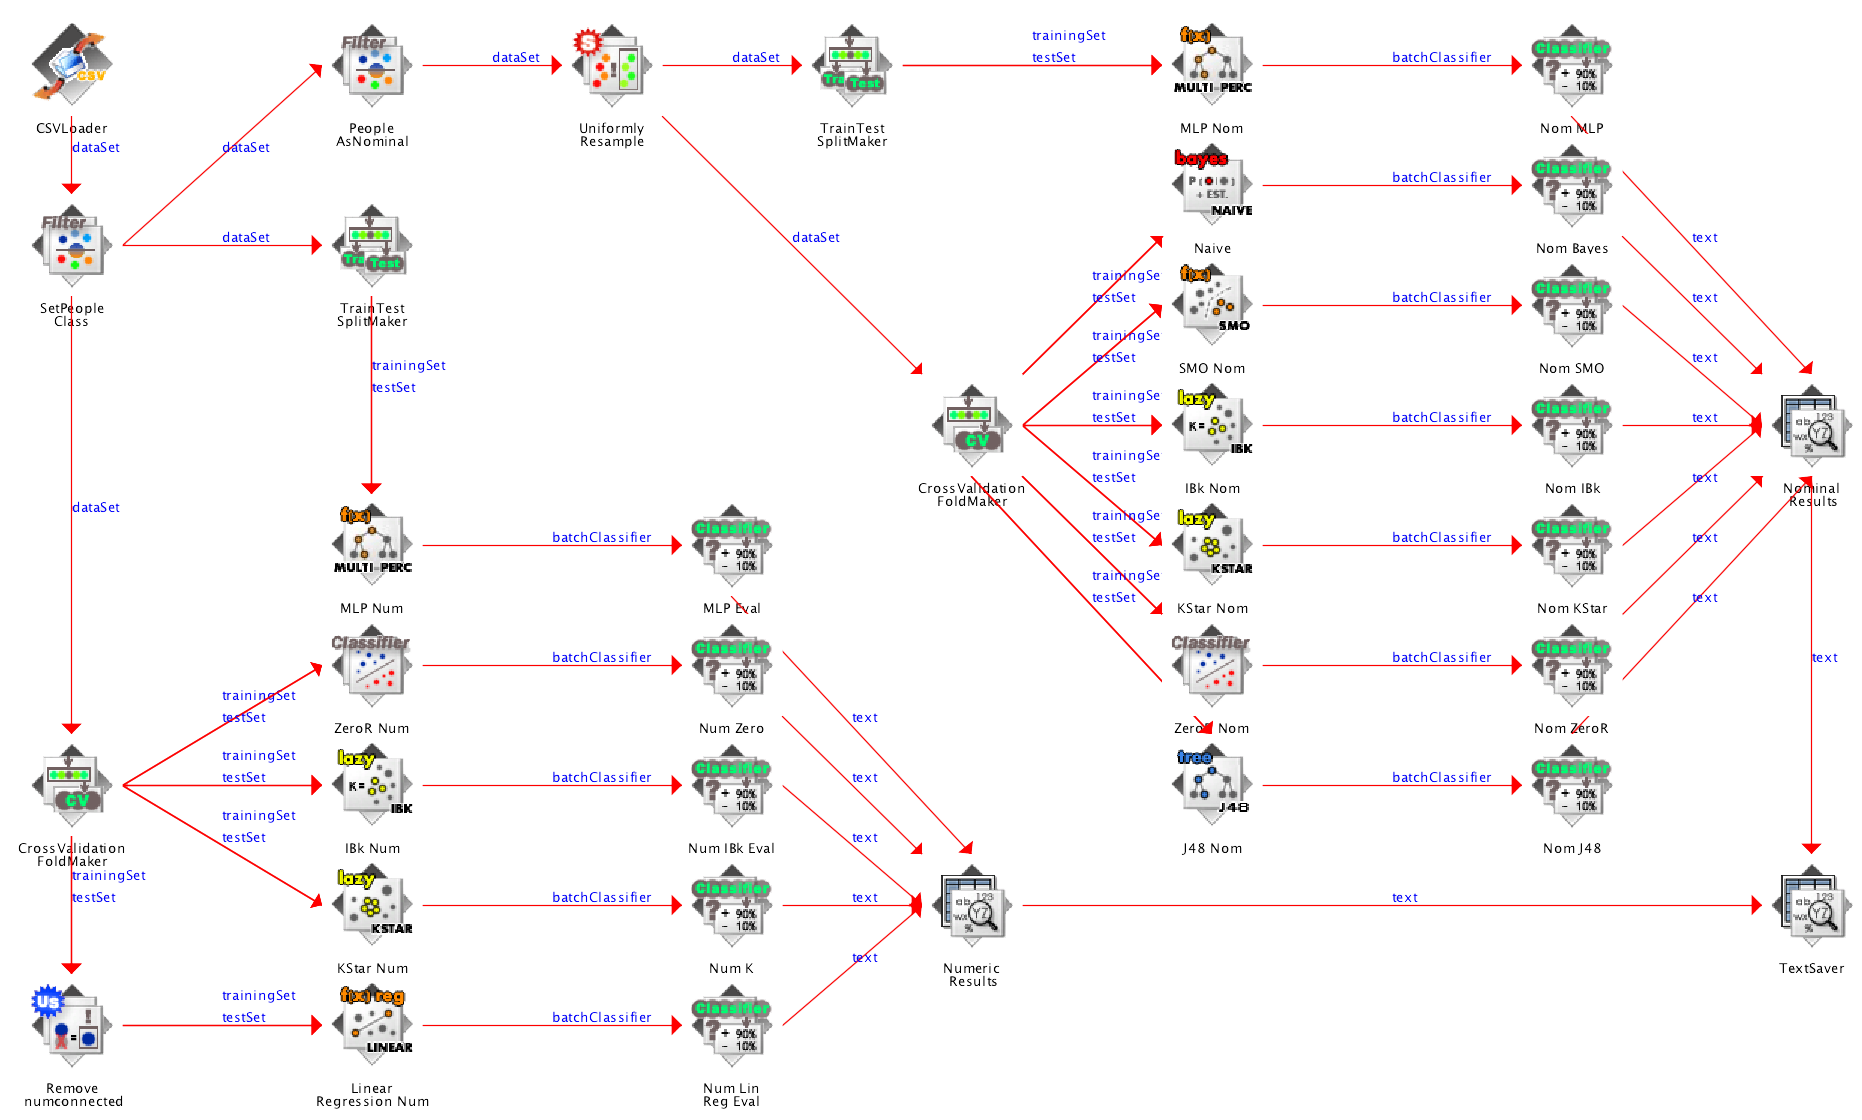
\includegraphics[width=0.95\linewidth]{../diagrams/unified-flow.png}
\caption{Unified Knowledge Flow for all experiments}
\label{fig:methods:unifiedflow}
\end{figure}
\end{landscape}


\subsection{Classifier Experiment Set 1 Setup}
In our first set of experiments, a scene was devised in accordance with \Fref{fig:exps:3setup} that attempted to sense people from above, as did Thermosense. The prototype was set up on the ceiling, pointing down at a slight angle. For ease of use, the prototype was powered by mains power, and was networked with a laptop for command input and data collection via Ethernet. This set of experiments involved between zero and three people being present in the scene, moving in and out in various ways in accordance with the script in \Fref{tab:exps:3script}.

\begin{table}
\centering
\begin{enumerate}
\item (Remained standing) One person walks in, stands in center, walks out of frame. (sub-experiment 1)
\item (Remained standing) One person walks in, joined by another person, both stand there, one leaves, then another leaves. (sub-experiment 2)
\item (Remained standing) One person walks in, joined by one, joined by another, all stand there, one leaves, then another, then another. (sub-experiment 3)
\item (Remained standing) Two people walk in simultaneously, both stand there, both leave simultaneously. (sub-experiment 4)
\item (Sitting) One person walks in, sits in center, moves to right, walks out of frame. (sub-experiment 5)
\item (Sitting) One person walks in, joined by another person, both sit there, they stand and switch chairs, one leaves, then another leaves. (sub-experiment 6)
\item (Sitting) One person walks in, joined by one, joined by another, they all sit there, one leaves, one shuffles position, then another leaves, then another. (x2) (sub-experiment 7, 8)
\item (Sitting) Two people walk in, both sit there, both leave. (sub-experiment 9)
\end{enumerate}
\caption{Experiment Set 1 Script}
\label{tab:exps:3script}
\end{table}

\begin{landscape}
 \begin{figure}
 \centering
 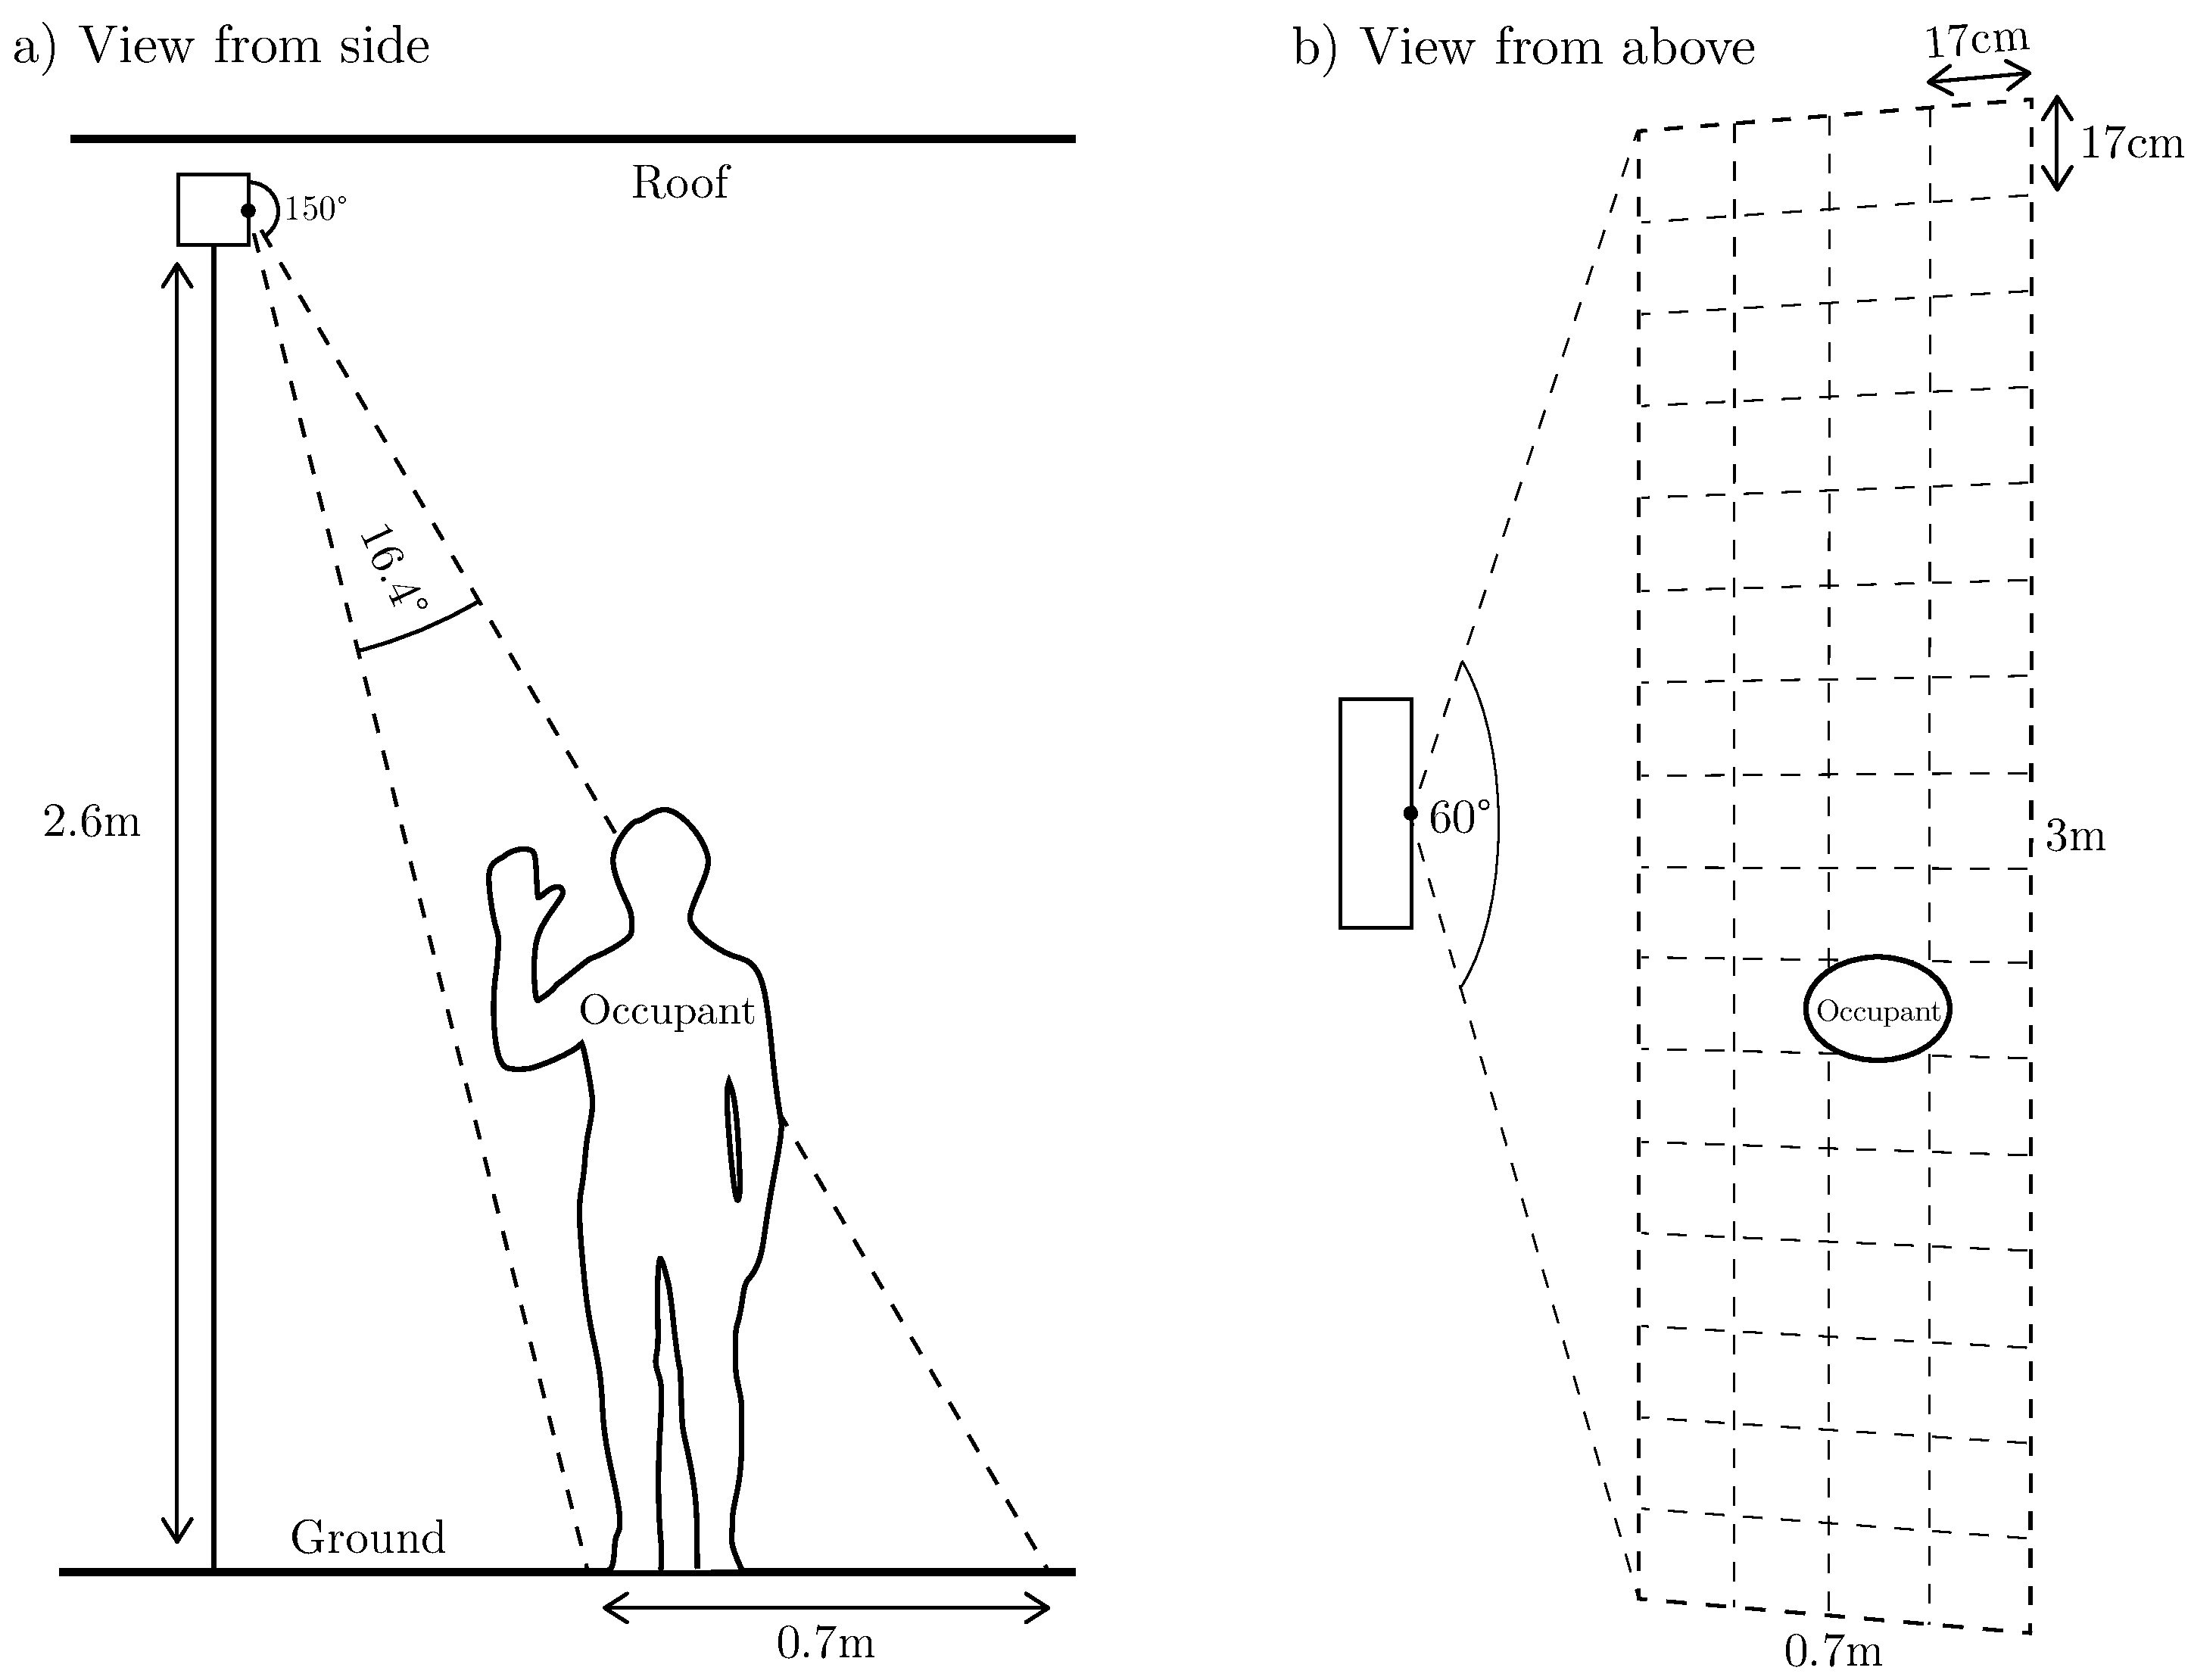
\includegraphics[height=\textheight]{../diagrams/third-exp-setup2.pdf}
 \caption{Classifier Experiment Set 1 Setup}
 \label{fig:exps:3setup}
 \end{figure}
\end{landscape}

In these experiments people moved slowly and deliberately, making sure there were large pauses between changes of action. The people involved were of average height, wearing various clothing. The room was cooled to 18 degrees for these experiments.

Each experiment was recorded with a thermal-visual synchronization at 1Hz over approximately 60-120 second intervals. Each experiment had 10-15 frames at the beginning where nothing was within the view of the sensor to allow the thermal background to be calculated. Each frame generated from these experiments was manually tagged with the ground truth value of its occupancy using the script mentioned previously.

The resulting features and ground truth were combined and exported to CSV allowing the Weka machine learning program to analyze them. This data was analyzed with the feature vectors always being considered numeric data and with the ground truth considered both numeric and nominal. All previously mentioned classification algorithms were run against the data set.

\section{Energy Efficiency Testing}

TODO: This section will contain experimental descriptions relating to the power consumption of the prototype.

 \ifcsdef{mainfile}{}{\bibliography{../references/primary}}
\end{document}
